\section{Hamilton--Jacobi formulation}
For deterministic dynamics $\dot x=f(t,x,u)$, running cost $\ell$ and
terminal cost $g$, a fixed feasible teacher $\phi$ has value
\begin{equation}
 V^\phi(t,x)=\int_t^T\ell(s,x_s^\phi,\phi(s,x_s^\phi))\,ds+g(x_T^\phi),
 \qquad J(\phi)=\E_{x_0}V^\phi(0,x_0).
\end{equation}
In a smooth region it satisfies policy evaluation,
\begin{equation}
 V_t^\phi+H(t,x,\phi,\nabla V^\phi)=0,
 \qquad H(t,x,u,p)=\ell(t,x,u)+p^\top f(t,x,u).
\end{equation}
The optimal HJB equation instead minimizes over actions:
\begin{equation}
 \partial_t V^*+\min_{u\in U}H(t,x,u,\nabla_xV^*)=0,
 \qquad V^*(T,x)=g(x).
\end{equation}
\begin{proposition}
Suppose $V^\phi$ is continuously differentiable along the relevant
trajectories, both feasible policies have well-defined trajectories and
integrable costs, and they share the initial distribution and terminal
cost. Then
\begin{align}
 J(\pi)-J(\phi)&=\E\int_0^T
 \mathcal A^\phi(t,x_t^\pi,\pi(t,x_t^\pi))\,dt,\\
 \mathcal A^\phi(t,x,u)&=H(t,x,u,\nabla V^\phi)
                  -H(t,x,\phi(t,x),\nabla V^\phi).
\end{align}
\end{proposition}
\begin{proof}
The chain rule and teacher evaluation equation give
$\ell(t,x_t^\pi,\pi)+\frac{d}{dt}V^\phi(t,x_t^\pi)
=\mathcal A^\phi(t,x_t^\pi,\pi)$. Integrate and use
$V^\phi(T,\cdot)=g$.
\end{proof}
Nonpositive integrated advantage implies no greater student cost. The
condition concerns student-visited states, which teacher samples alone
need not cover.


For $x_{t+1}=F_t(x_t,u_t)$, the discrete counterpart is
\begin{align}
 A_t^\phi(x,u)&=c_t(x,u)+V_{t+1}^\phi(F_t(x,u))-V_t^\phi(x),\\
 J(\pi)-J(\phi)&=\E_{x_0}\sum_{t=0}^{H-1}
 A_t^\phi(x_t^\pi,\pi_t(x_t^\pi)).
\end{align}
Differentiating the fixed teacher's feedback trajectory gives
\begin{equation}
 p_t=c_x+(D_x\phi_t)^\top c_u+
       (F_x+F_uD_x\phi_t)^\top p_{t+1},\qquad p_H=\nabla g.
\end{equation}
One reverse sweep obtains the covectors without a state-space grid or
fitted scalar critic~\cite[Sec.~3, Eq.~(3)]{heess2015svg}. At projection
boundaries, automatic differentiation uses the implemented branch.

\subsection{Feasible targets}
For control-affine dynamics and isotropic quadratic action cost, write
\begin{equation}
 F_t(x,u)=a_t(x)+B_tu,\quad
 c_t(x,u)=c_{0t}(x)+r_t\|u\|^2+l_t^\top u,\quad
 b_t=l_t+B_t^\top p_{t+1}.
\end{equation}
The local Bellman model is $q_t(u)=r_t\|u\|^2+b_t^\top u$, up to
an action-independent constant. For Euler dynamics $F=x+hf$ and
$c=h\ell$, $q_t/h$ is the control-dependent Hamiltonian with frozen
next-state covector. For closed convex $U$ and $r_t>0$,
\begin{align}
 u_t^+&=\arg\min_{u\in U}\{q_t(u)+\tfrac\rho2\|u-u_t^\phi\|^2\},\\
 &=\operatorname{proj}_U\frac{\rho u_t^\phi-b_t}{2r_t+\rho}.
\end{align}
Anisotropic costs require metric projection. The same local expansion
is used at the final decision; its terminal remainder need not vanish.
For fixed state and teacher action, nonexpansivity gives
\begin{equation}
 \|u^+(\widehat p)-u^+(p)\|
 \leq\frac{\|B^\top(\widehat p-p)\|}{2r+\rho}.
\end{equation}

\subsection{Information lost at constraints}
Put $Q_\rho=q+\rho\|u-u^\phi\|^2/2$ and $a=r+\rho/2$. Then
\begin{equation}\label{eq:v9-normal}
 Q_\rho(u)-Q_\rho(u^+)=a\|u-u^+\|^2+
              \nabla Q_\rho(u^+)^\top(u-u^+).
\end{equation}
The normal term is nonnegative on $U$ and vanishes for an interior
target. For a ball, if both actions lie on its sphere and
$\nabla Q_\rho(u^+)=-\lambda u^+$, the difference becomes
$(a+\lambda/2)\|u-u^+\|^2$. General feasible students require the
additional term derived below.
\subsection{Identical labels, different costs}\label{sec:information-loss}
\begin{proposition}\label{prop:label-loss}
Exact one-step Bellman models can have identical strictly improving
targets and identical globally optimal target fits with opposite
teacher-relative cost effects, even with common quadratic curvature,
complete coverage and a teacher in the student class.
\end{proposition}
\begin{proof}
Take three equiprobable contexts, $U=[-1,1]$, teacher zero and constant
students $u=c$. Let
\begin{equation}\label{eq:witness-cost}
 Q_i(u)=(u-\mu_i)^2,\qquad (\mu_1,\mu_2,\mu_3)=(\tau,-1,-1),\quad \tau\geq1.
\end{equation}
For $\rho=0$, the targets are $(1,-1,-1)$ and each improves its teacher.
Their unique minimum-MSE fit is $c=-1/3$, with MSE $8/9<1$. However,
\begin{equation}\label{eq:witness-gap}
 J(-1/3)-J(0)=\frac{2\tau-3}{9},
\end{equation}
which is negative at $\tau=1$ and positive for $\tau>3/2$.

An exact Bellman realization uses $x=(s,y)$, $F(s,y,u)=(s,u)$,
$c_t=u^2$, and $g(s,y)=\mu(s)^2-2\mu(s)y$, with
$\mu(s)=-1+(\tau+1)(s-2)(s-3)/2$. Start uniformly at $(s,0)$,
$s\in\{1,2,3\}$. Total cost is Eq.~\eqref{eq:witness-cost}; the
projected terminal covector is $-2\mu_i$. Sensitivity error and
continuation remainder both vanish.
\end{proof}

At $\tau=10$, the discarded normal term is $18(1-u)$ in the first
context and zero elsewhere. Teacher cost is 34, best target-fit cost
is $323/9=35.888889$, and direct cost minimization in the same constant
class selects $c=1$ with cost $89/3=29.666667$.
For any fixed finite $\rho\geq0$, replacing $\mu_i$ by
$\beta(\tau,-1,-1)_i$, $\beta=1+\rho/2$, keeps the proximal targets
unchanged and gives fitted cost difference $[1+2\beta(\tau-2)]/9>0$
at $\tau=10$. This is an existence construction for each fixed $\rho$.

Retaining $a_z=r_z+\rho_z/2$ and $n_z=\nabla Q_{\rho,z}(u_+)$ restores
\begin{equation}\label{eq:cost-preserving-loss}
 L_{\rm cost}(u;z)=a_z\|u-u_+\|^2+n_z^\top(u-u_+)
                 =Q_{\rho,z}(u)-Q_{\rho,z}(u_+).
\end{equation}
For a fixed state distribution and a class containing the teacher, a
global minimizer cannot increase mean proximal model value. The
teacher's zero proximal penalty gives the same conclusion for the
unregularized model. This is a policy-cost comparison in the exact
one-step example; nonlinear continuation and changed occupancy require
the bounds in \ref{app:transfer}.

On $U=\{u:\|u\|\leq R\}$, write $n_z=-\lambda_z u_+$,
$\lambda_z\geq0$, with $\lambda_z=0$ for interior targets. Expansion gives
\begin{equation}\label{eq:radial-information}
 L_{\rm cost}(u;z)=(a_z+\lambda_z/2)\|u-u_+\|^2
                  +\frac{\lambda_z}{2}(R^2-\|u\|^2).
\end{equation}
Weighted action fitting omits the second term. It can therefore miss
the cost of a student's interior compromise even with the correct weight.

\begin{figure}[htbp]\centering
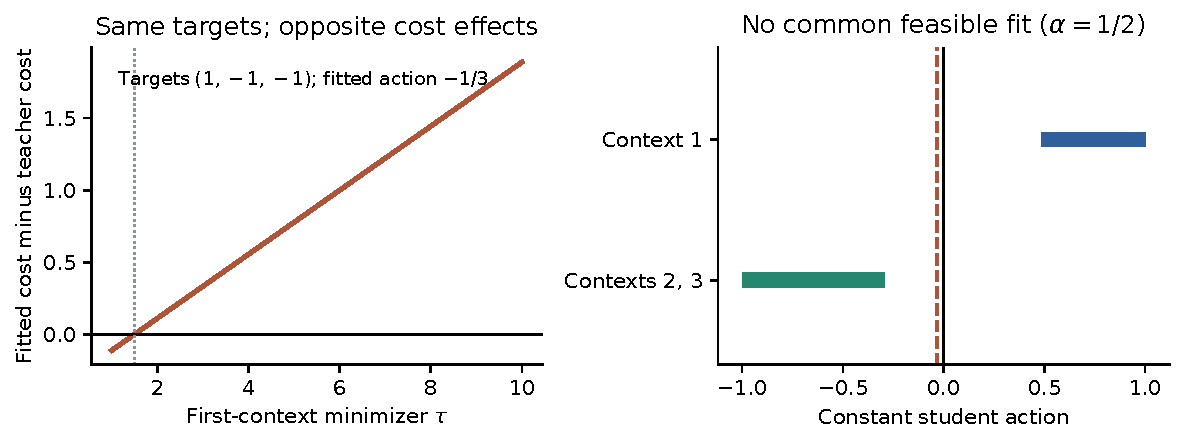
\includegraphics[width=\linewidth]{figures/teaching_information_loss_corrected.pdf}
\caption{Exact constructed failures of the teaching interface. Left:
the same constrained action targets and the same best constant fit have
opposite cost effects as the unconstrained minimizer $\tau$ changes,
with quadratic curvature fixed. Right: each
improvement set is nonempty, but their intersection is empty; the dashed
line is the best constant set-distance fit (\ref{sec:joint-sets}). }
\label{fig:information-loss}
\end{figure}

